% Preamble
\documentclass[a4paper, 12pt]{article}
\usepackage[margin=1in]{geometry} % Set margin
\usepackage{pdfpages} % Insert pdf pages
\usepackage{amssymb,amsmath,amsthm, amsfonts} % Math libraries

% Custom commands
\newcommand{\sub}[1]{\subsection{\underline{#1}}}
\newcommand{\subsub}[1]{\subsubsection{\underline{#1}}}
\newcommand{\R}{\ensuremath{\mathbb{R}}}
\newcommand{\F}{\ensuremath{\mathbb{F}}}
\newcommand{\N}{\ensuremath{\mathbb{N}}}
\newcommand{\Onef}{\ensuremath{1_{\F}}}
\newcommand{\Zerof}{\ensuremath{0_{\F}}}
\newcommand{\eqbcuz}[1]{\text{~$\stackrel{(#1)}{=}$~}}
\newcommand{\eq}[1]{\begin{align*}#1\end{align*}}
\newcommand{\eqn}[1]{\begin{align}#1\end{align}}
\newcommand{\set}[1]{\big{\{} #1 \big{\}}}
\renewcommand{\qed}{\hfill\(\qedsymbol\)}
\newtheorem{lemma}{Lemma}

% Begin Document %
\begin{document}

% Title Page
\begin{titlepage}
    %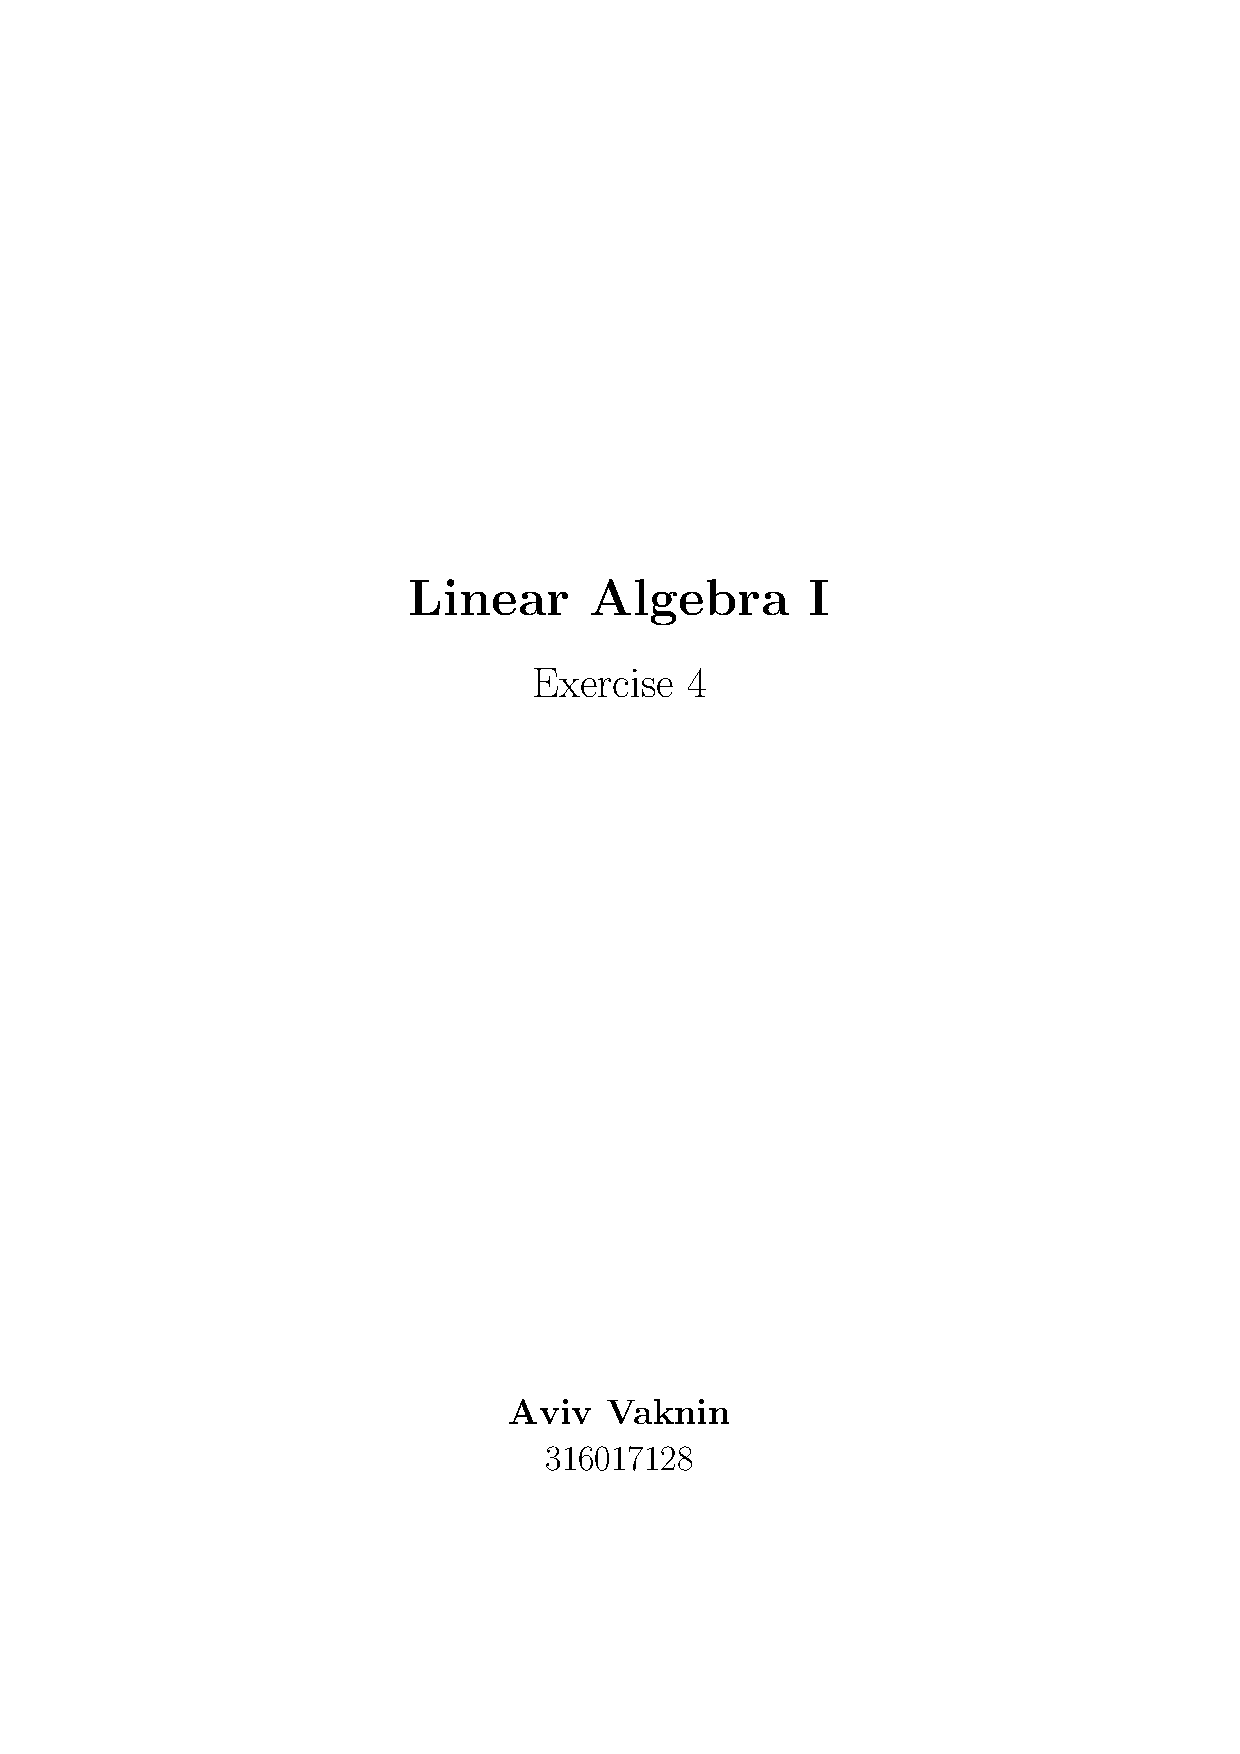
\includepdf{title.pdf}
\end{titlepage}

% 3
\setcounter{section}{2}
\section{Calculate \textit{AC}, \textit{BC}, \textit{ABC} and \textit{BAC}}
\eq{
    AC=\begin{bmatrix}
        c^1_1 & c^1_2 & c^1_3 \\
        c^3_1 & c^3_2 & c^3_3 \\
        c^2_1 & c^2_2 & c^2_3
    \end{bmatrix}
    \\
    BC=\begin{bmatrix}
        c^3_1 & c^3_2 & c^3_3 \\
        c^1_1 & c^1_2 & c^1_3 \\
        c^2_1 & c^2_2 & c^2_3
    \end{bmatrix}
    \\
    A(BC)=\begin{bmatrix}
        c^3_1 & c^3_2 & c^3_3 \\
        c^2_1 & c^2_2 & c^2_3 \\
        c^1_1 & c^1_2 & c^1_3
    \end{bmatrix}
    \\
    B(AC)=\begin{bmatrix}
        c^2_1 & c^2_2 & c^2_3 \\
        c^1_1 & c^1_2 & c^1_3 \\
        c^3_1 & c^3_2 & c^3_3
    \end{bmatrix}
}

% 6
\setcounter{section}{5}
\section{Prove that \eq{A(\lambda{B})=B(\lambda{A})=\lambda(AB)}}
We'll prove this by showing:
\eq{
    [A(\lambda{B})]^i_j=[B(A\lambda)]^i_j=[\lambda(AB)]^i_j
}
Therefore, if for all of the matrices, all of the cells are identical, the matrices are the same.
\eq{
    &[A(\lambda{B})]^i_j=\sum^n_{k=1}a^i_k(b^k_j\lambda)\\
    &[B(A\lambda)]^i_j=\sum^n_{k=1}b^k_j(a^i_k\lambda)\\
    &[\lambda(AB)]^i_j=\lambda(\sum^n_{k=1}a^i_kb^k_j)
}
As all of the operations are happening inside $\F$, we can factor the $\lambda$, and therefore:
\eq{
    &[A(\lambda{B})]^i_j=\sum^n_{k=1}a^i_k(b^k_j\lambda)=\lambda(\sum^n_{k=1}a^i_kb^k_j)\\
    &[B(A\lambda)]^i_j=\sum^n_{k=1}b^k_j(a^i_k\lambda)=\lambda(\sum^n_{k=1}a^i_kb^k_j)
}
Therefore, we've shown that:
\eq{
    [A(\lambda{B})]^i_j=[B(A\lambda)]^i_j=[\lambda(AB)]^i_j
}
And therefore:
\eq{
    A(\lambda{B})=B(\lambda{A})=\lambda(AB)
}
\qed

% 7
\section{Prove that \eq{A(\lambda{C}+D)=O}}
According to question \textbf{5}:
\eq{
    A(\lambda{C}+D)=A\lambda{C}+AD
}
According to question \textbf{6}:
\eq{
    A\lambda{C}+AD=\lambda\cdot{AC}+AD
}
It is given that $AC=AD=O$, therefore:
\eq{
    \lambda\cdot{AC}+AD=\lambda\cdot{O}+O
}
According to the properties of matrix scalar multiplication:
\eq{
    a\cdot{O}=O
}
Therefore:
\eq{
    \lambda\cdot{O}+O=O+O=O
}
\qed

% 10
\setcounter{section}{9}
\section{}
\eq{
    A=&\begin{bmatrix}
        0 & 1\\
        0 & 0
    \end{bmatrix}
    \\
    A^2=&\begin{bmatrix}
        0 & 1\\
        0 & 0
    \end{bmatrix}
    \begin{bmatrix}
        0 & 1\\
        0 & 0
    \end{bmatrix}
    =
    \begin{bmatrix}
        0 & 0\\
        0 & 0
    \end{bmatrix}
}

% 11
\section{Calculate $A^{2020}$
    \eq{
        A=\begin{bmatrix}
            1 & 1\\
            0 & 1
        \end{bmatrix}
    }
}
We've proved in question \textit{16A} $\forall{a,b}\in\F$:
\eq{
    \begin{bmatrix}
        1 & a\\
        0 & 1
    \end{bmatrix}
    \begin{bmatrix}
        1 & b\\
        0 & 1
    \end{bmatrix}
    =
    \begin{bmatrix}
        1 & a+b\\
        0 & 1
    \end{bmatrix}
}
Therefore, we can see that:
\eq{
        A^n=\begin{bmatrix}
            1 & 2^{n-1}\\
            0 & 1
        \end{bmatrix}
        \\
        A^{2020}=\begin{bmatrix}
            1 & 2^{2019}\\
            0 & 1
        \end{bmatrix}
}
\pagebreak

% 14
\setcounter{section}{13}
\section{}
We'll prove this using induction over the sequence's length as \textit{\textbf{s}}.
\subsub{$s=1$:}
If the sequence's length is 1, it is trivial that the statement is true, as ${A}_1\in{GL}_n(\F)$.\\
That is because $A_1=A_1$, and $(A_1)^{-1}=(A_1)^{-1}$.
\subsub{$s=s-1$:}
We'll assume the statement is true for any sequence of an arbitrary length \textit{\textbf{s-1}}, and we'll mark it as \textit{\textbf{B}}, that is:
\eq{
    &B=A_1\cdot...\cdot{A}_{s-1}\in{GL}_n(\F)\\
    &B^{-1}=(A_1\cdot...\cdot{A}_{s-1})^{-1}=A_{s-1}^{-1}\cdot...\cdot{A}_{1}^{-1}
}
\subsub{$s=s$:}
Now, we'll prove the statement is true for a sequence with length \textit{\textbf{s}}.\\
Let $A_s$ equal to the identity matrix of size \textit{n}:
\eq{
    A_s=\mathbb{I}_n
}
Now, we can prove ($A_1\cdot...\cdot{A}_s)\in{GL}_n(\F)$:
\eq{
    &A_1\cdot...\cdot{A}_s=B\cdot{A}_{s}\\
    &=B\cdot\mathbb{I}_n\\
    &=B\\
    &B\in{GL}_n(\F)\\
    &A_1\cdot...\cdot{A}_s\in{GL}_n(\F)
}
Let's show that $(A_1\cdot...\cdot{A}_{s})^{-1}=B^{-1}$:
\eq{
    &(A_1\cdot...\cdot{A}_{s})^{-1}=(A_1\cdot...\cdot{A}_{s-1}\cdot{A}_{s})^{-1}\\
    &=(B\cdot{A}_{s})^{-1}\\
    &=(B\cdot\mathbb{I}_n)^{-1}\\
    &=B^{-1}\\
}
Now, using the fact that ${A}_{s}=\mathbb{I}_n={A}_{s}^{-1}$, we'll show that ${A}_{s}^{-1}\cdot...\cdot{A}_{1}^{-1}=B^{-1}$:
\eq{
    &{A}_{s}^{-1}\cdot...\cdot{A}_{1}^{-1}={A}_{s}^{-1}\cdot{A}_{s-1}^{-1}\cdot...\cdot{A}_{1}^{-1}\\
    &={A}_{s}^{-1}\cdot{B}^{-1}\\
    &=\mathbb{I}_n\cdot{B}^{-1}\\
    &={B}^{-1}\\
}
Now, we can conclude:
\eq{
    (A_1\cdot...\cdot{A}_{s})^{-1}={B}^{-1}={A}_{s}^{-1}\cdot...\cdot{A}_{1}^{-1}
}
\qed\pagebreak

% 17
\setcounter{section}{16}
\section{}
\sub{$\implies$:}
It is given that \textit{C} is invertible, therefore $det(C)\neq{0}$, that is:
\eq{
    &det(C)=A\cdot{B}-O\cdot{O}\\
    &=AB\neq{O}
}

% 19
\setcounter{section}{18}
\section{Prove \textit{A} is reversible\eq{
    A^3-2A+I=O
}}
We'll start by deducting $I$ and multiplying the equation by $(-I)$:
\eq{
    2A-A^3&=I\\
    A(2I-A^2)&=I\\
    A(\sqrt{2}I+A)(\sqrt{2}I-A)&=I
}
\textit{A} is reversible if and only if there exists $A^{-1}$ such that $AA^{-1}=I$, therefore:
\eq{
    A^{-1}=(\sqrt{2}I+A)(\sqrt{2}I-A)
}
\qed

% End Document %
\end{document}